\subsection{Struktur der Proben}

Alle in diesem Versuch untersuchten Materialien (Gold,Graphit und eine unbekannte Probe) sind Leiter, sie unterscheiden sich jedoch in der Konfiguration der Elektronen. Es gibt einen unterschied zwischen der Verteilung der Elektronen in Metallen und Halbleitern. Metalle werde dabei durch das Elektronen-Gas beschrieben und somit eine homogen Verteilung angenommen wird. Bei der Beschreibung von Halbleitern m�ssen noch Bandl�cken ber�cksichtigt werden. Da die r�umliche Verteilung der Elektronen nicht homogen ist, kann aus der Ladungsverteilung die Position der Atome bestimmt werden. Es soll nun genauer auf die beiden bekannten Proben Gold und Graphit eingegangen werden.

\subsubsection{Graphit}

Die Graphitporbe ist ein HOPG (Highly orderd pyrolytic graphit), ein Halbleiter mit einer hcp-Gitterstruktur. In Abbildung \ref{fig:graphit} ist die Gitterstruktur des Graphit zu sehen. In einer Ebene werden die Kohlenstoffatome aufgrund der sp2-Hybirdisirung  stark durch kovalente Bindungen zusammengehalten. Zwischen den Ebenen werde die Kohlenstoffatome nur von Van-der-Waals-Kr�ften zusammengehalten. 

\begin{figure}[H]
	\centering
  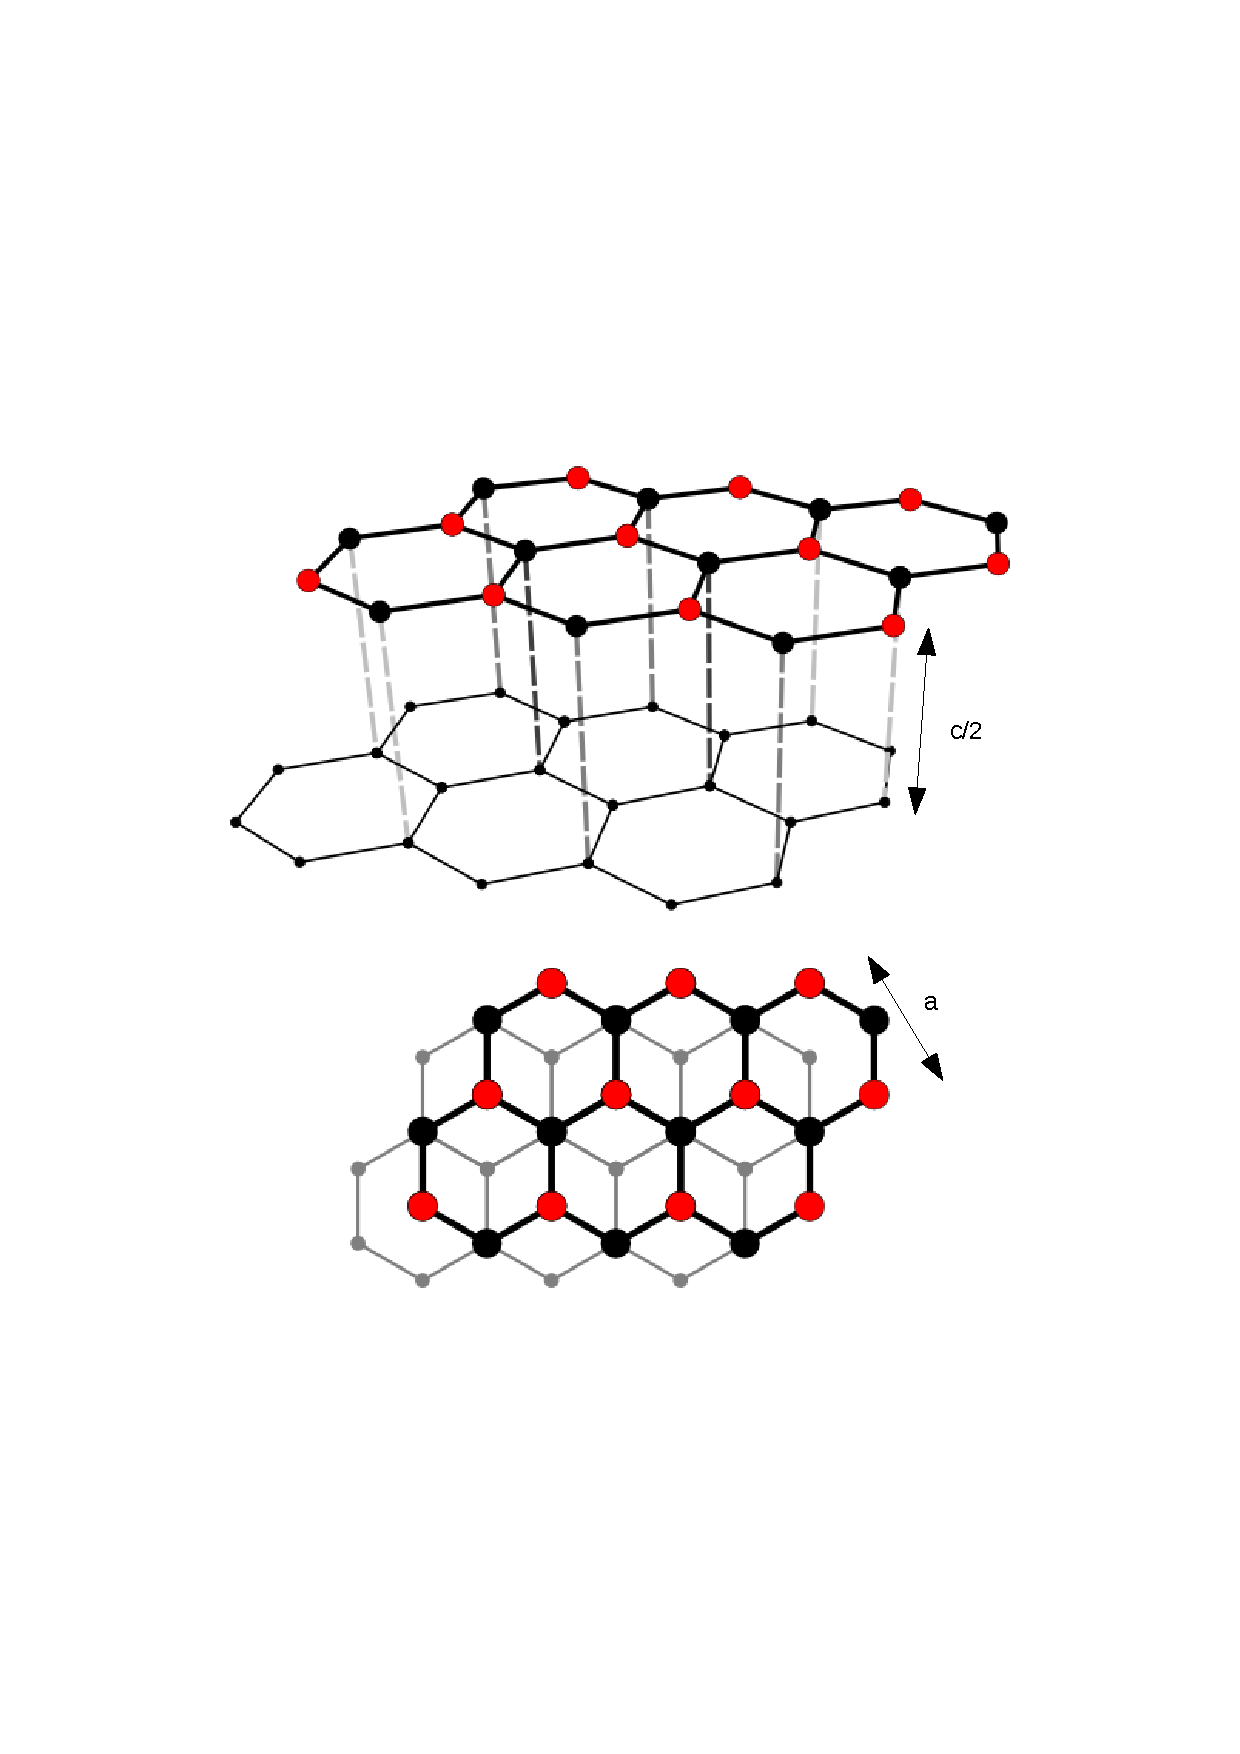
\includegraphics[trim = 10mm 70mm 30mm 60mm, clip,scale=0.8]{graphit.pdf}
	\caption{Schematische Struktur von Graphit. Die Ebenen liegen im ABAB-Form vor, sodass immer die jede zweite gleich aufliegt. Die Ebenen untereinander besitzen nur an jedem zweitem Punkt der Hexagonale eine Verbindung. Entnommen von \cite{graphit-bild}, modifiziert}
	\label{fig:graphit}
\end{figure}

Die in Abbildung \ref{fig:graphit} eingezeichneten Gitterkonstanten haben die Werte a = \SI{2,26}{\angstrom} und c = \SI{6,71}{\angstrom} (vgl. \cite{graphit}). Aufgrund ABAB-Form liegen immer drei Atome in den Hexagonalen etwas erh�ht und haben so eine h�here frei elektrische Zustandsdichte. Diese Struktur ist auch mit dem RTM zu sehen.

\subsubsection{Gold}
Gold hat eine fcc-Kristallstruktur, dabei betr�gt die Gitterkonstante a = \SI{4.065}{\angstrom}  \cite{PhysRev.25.753}. Untersucht wird die (111)-Goldschicht, dabei sind (111) die Millerindizes, die die r�umliche Struktur des Kristalls beschreiben. Es ist deutlich schwerer die atomare Struktur von Gold zu messen, da die Atome homogen verteilt sind.